\documentclass[../TG_magistrsko_delo_sections.tex]{subfiles}
\graphicspath{{\subfix{../images/}}}

\begin{document}
Po zaklučenem dokazu si lahko postavimo vprašanje, kako se spremenijo posledice v izreku, če spremenimo predpostavke izreka. Glede na to, kako spremenimo predpostavke, lahko pridemo do različnih posplošitev izreka. V primeru izreka Šarkovskega obstaja več posplošitev. Nekatere obravnavajo izrek za nezvezne funkcije, ki ustrezajo določenim pogojem, druge pa preučujejo zvezne funkcije, ki so definirane na različnih topoloških prostorih. Vprašamo se lahko, kakšna ureditev naravnih števil, če ta obstaja, opiše prisotnost periodičnih točk zvezne funkcije $f:X \to X$, ki slika nek topološki prostor $X$ nazaj vase. Natančneje, iščemo relacijo $\triangleleft_X$ z lastnostjo: če je $m$ perioda za zvezno funkcijo $f:X \to X$, potem je vsako naravno število $l$, za katero je $l \triangleleft_X m$, tudi perioda za funkcijo $f$. Če je relacija $\triangleleft_X$ enaka relaciji Šarkovskega, ki smo jo spoznali v definiciji~\ref{def:ureditev-sark}, pravimo, da je prostor $X$ \emph{prostor Šarkovskega}. To poglavje bomo namenili temu, da bomo spoznali nekaj prostorov Šarkovskega in tudi nekaj prostorov, ki to niso. S primeri in protiprimeri bomo poskušali ugotoviti katere topološke lastnosti imajo prostori Šarkovskega.
Preden začnemo s preučevanjem različnih prostorov Šarkovskega se prepričajmo, da je lastnost biti prostor Šarkovskega tudi topološka lastnost. 
\begin{trditev}
Lastnost biti prostor Šarkovskega je topološka lastnost. To pomeni, če je $X$ prostor Šarkovskega in je prostor $Y$ homeomorfen prostoru $X$, potem je tudi $Y$ prostor Šarkovskega.
\end{trditev}
\begin{proof}
Naj bo prostor $X$ prostor Šarkovskega in naj bo prostor $Y$ homeomorfen prostoru $X$. Naj bo $h : X \to Y$ homeomorfizem med prostoroma $X$ in $Y$. Funkciji $f : Y \to Y$ in $g = h^{-1} \circ f \circ h : X \to X$ imata enake periode, zato je $Y$ tudi prostor Šarkovskega.
\end{proof}

Nove prostore, ki so prostori Šarkovskega, lahko poiščemo tudi s pomočjo nekaterih zveznih preslikav. Definirajmo eno tako preslikavo, ki nam pomaga konstruirati nove prostore Šarkovskega.
\begin{definicija}
Naj bo $X$ topološki prostor in $A \subseteq X$ njegov podprostor. Zvezni preslikavi $r : X \to A$ pravimo \emph{retrakcija}, če je preslikava $r|_A = id_A$. Podprostor $A \subseteq X$ je \emph{retrakt} prostora $X$, če obstaja retrakcija $r: X \to A$.
\end{definicija}

S pomočjo retrakcije lahko pridemo do novih prostorov Šarkovskega.

\begin{trditev}
Retrakt prostora Šarkovskega je prostor Šarkovskega.
\end{trditev}
\begin{proof}
Denimo, da je prostor $X$ prostor Šarkovskega in prostor $A \subseteq X$ retrakt prostora $X$. Naj bo $r : X \to A$ retrakcija $i : X \to A$ inkluzija. Če je funkcija $f : A \to A$ zvezna, ima funkcija $g = i \circ f \circ r : X \to X$ enake periodične točke, kot funkcija $f$. Zato je tudi prostor $A$ prostor Šarkovskega.
\end{proof}

Sedaj pa si poglejmo nekaj primerov prostorov Šarkovskega. Iz prejšnjih poglavji je razvidno, da so tipični predstavniki prostorov Šarkovskega množica realnih števil in intervali v realnih številih. Poglejmo si primer prostora, ki ni prostor Šarkovskega.

\begin{primer}
Krožnica $S^1 = \{ (cos(\varphi), \sin(\varphi)), \varphi \in [0, 1) \}$ ni prostor Šarkovskega. Hitro se lahko prepričamo, da obstajajo funkcije, ki imajo samo eno periodo. To so rotacije okoli koordinatnega izhodišča. Definiramo družino funkciji: 
\begin{equation*} %\label{eq1}
\begin{split}
R_n &: S^1 \to S^1 \\ 
R_n &: (cos(\varphi), \sin(\varphi)) \mapsto (cos(\varphi + \frac{2 \pi}{n}), \sin(\varphi + \frac{2 \pi}{n})).
\end{split}
\end{equation*}
Vse točke krožnice $S^1$ so periodične točke za funkcijo $R_n$ in vse imajo periodo $n$. Zato iz obstoja periodične točke za zvezno funkcijo $f : S^1 \to S^1$ ne moremo sklepati na obstoj drugih period za to funkcijo.
\end{primer}
S podobnim sklepanjem kot zgoraj lahko za nekatere prostore hitro preverimo, da niso prostori Šarkovskega. To naredimo tako, da poiščemo kakšno os $n$-kratne rotacijske simetrije, kjer je $n$ naravno število večje od $2$. Pri takih primerih lahko hitro ugotovimo, da ima rotacija neko periodo večjo od $2$, nima pa periode $2$. Zaradi tega taki prostori ne morejo biti prostori Šarkovskega. Primeri takih prostorov so npr. sfera, krogla, torus \dots 

Videli smo, da pri krožnici ne obstaja taka relacija, ki bi opisala periode zveznih funkcij iz prostora $S^1$ nazaj v prostor $S^1$. V naslednjem primeru bomo spoznali prostor, ki ni prostor Šarkovskega, vseeno pa lahko iz prisotnosti nekaterih period sklepamo na prisotnost durgih.
\begin{primer}
Naj bo prostor $X$ unija dveh disjunktnih intervalov: $X = [-2, -1] \cup [1, 2]$. Funkcija $g : X \to X$ podana s predpisom $g(x) = -x$ je zvezna funkcja. Vsaka točka iz prostora $X$ ima periodo 2, funkcija pa nima fiksne točke, zato prostor $X$ ni prostor Šarkovskega. Vseeno lahko poiščemo relacijo $\triangleleft_X$, ki opiše katere periode ima lahko funkcija. Zaradi lažje obravnave bomo interval $[-2, -1]$ označili z $I_1$, interval $[1, 2]$ pa z $I_2$. Pri poljubni funkciji $f: X \to X$ imamo štiri možnosti. Če je $f(I_1) \subseteq I_1$ in $f(I_2) \subseteq I_2$ lahko za funkciji $f|_{I_1}$ in $f|_{I_2}$ uporabimo izrek Šarkovskega in ugotovimo, de je relacija $\triangleleft_X$ enaka relaciji Šarkovskega. V primeru, ko je $f(I_1) \subseteq I_1$ in $f(I_2) \subseteq I_1$ lahko periodične točke ležijo samo v intervalu $I_1$. Za funkcijo $f|_{I_1}$ uporabimo izrek Šarkovskega in ugotovimo, da je relacija $\triangleleft_X$ enaka relaciji Šarkovskega. Podoben sklep lahko naredimo tudi v primeru, ko je $f(I_1) \subseteq I_2$ in $f(I_2) \subseteq I_2$. Drugače je v primeru $f(I_1) \subseteq I_2$ in $f(I_2) \subseteq I_1$. V tem primeru se točke iz intervala $I_1$ s funkcijo $f$ slikajo v interval $I_2$ in obratno. Zato ima vsaka periodična točka sodo periodo. Naj bo $x \in X$ točka periode $2m$ za funkcijo $f$. Brez izgube splošnosti lahko sklepamo, da točka $x$ pripada intervalu $I_1$. Potem ima točka $x$ periodo $m$ za funkcijo $f^2|_{I_1} :I_1 \to I_1$. Ker je $I_1$ prostor Šarkovskega in je $f^2$ zvezna funkcija, lahko uporabimo izrek Šarkovskega in ugotovimo, da za vsako naravno število $l$, za katerega velja $l \triangleleft m$, obstaja točka $y \in I_1$ s periodo $l$ za funkcijo $f^2$. Točka $y$ ima periodo $2l$ za funkcijo $f$, saj je orbita točke $y$ sestavljena iz $l$ različnih točk v intervalu $I_1$ (sode iteracije) in $l$ različnih točk iz intervala $I_2$ (lihe iteracije). 
Ugotovili smo naslednje: Če ima zvezna funkcija $f:X \to X$ liho periodo $m$, potem ima zagotovo tudi vse periode $l$, kjer je $l \triangleleft m$. Če pa je perioda $m$ soda, potem ima funkcija vse periode $l\neq1$, za katere je $l \triangleleft m$. 
Dobimo relacijo $\triangleright_X$:
$$3 \triangleright_X 5 \triangleright_X 7 \triangleright_X \cdots \triangleright_X 2\cdot 3 \triangleright_X 2\cdot 5 \triangleright_X 2\cdot 7 \triangleright_X \cdots \triangleright_X 2^2\cdot 3 \triangleright_X 2^2\cdot 5 \triangleright_X 2^2\cdot 7 \triangleright_X \cdots \triangleright_X 2^3 \triangleright_X 2^2 \triangleright_X 2,$$
$$3 \triangleright_X 5 \triangleright_X 7 \triangleright_X \cdots \triangleright_X 1.$$
\end{primer}

Na začetku primera smo enostavno pokazali, da disjunktna unija dveh intervalov ni prostor Šarkovskega. Z zelo podobno idejo lahko pokažemo, da je vsak prostor Šarkovskega povezan.

\begin{trditev}
Prostor Šarkovskega je povezan.
\end{trditev}
\begin{proof}
Naj bo prostor $X$ disjunktna unija prostorov $A$ in $B$ in naj bosta $a \in A$ in $b \in B$ poljubni točki tega prostora. Definiramo funkcijo $f:X \to X$ s predpisom:
\[ f(x) = \begin{cases}
  a, & \mbox{ če $x \in B $}\\
  b ,& \mbox{ če $x \in A$.}
  \end{cases}
  \]
Funkcija $f$ ima samo dve periodični točki. To sta točki $a$ in $b$. Obe pa imata periodo 2. Ker nobena točka prostora $X$ ni fiksna točka za funkcijo $f$, prostor $X$ ni prostor Šarkovskega.
\end{proof}




Prepričali smo se že, da je vsak prostor Šarkovskega povezan prostor. V nadaljevanju bomo ponovili kakšni prostori so lokalno povezani in ugotovili, da je prostor Šarkovskega lahko lokalno nepovezan prostor.

\begin{definicija}
Prostor $X$ je lokalno povezan prostor, če za vsako točko $x \in X$ in vsako odptro množico $U \subseteq X$, ki vsebuje točko $x$, obstaja taka odprta povezana množica $V \subseteq X$, da je $x \in V \subseteq U$. Prostoru, ki ni lokalno povezan pravimo lokalno nepovezan prostor.
\end{definicija}

poglejmo si nekaj primerov:
\begin{primer}
Odprti disk v $\R^2$ je povezan in lokalno povezan prostor.
\end{primer}

\begin{primer}
Poglejmo si nepovezan prostor, sestavljen iz treh komponent za povezanost kot prikazuje slika. Prostor je lokalno povezan, saj za vsako točko $x \in X$ in vsako njeno odprto okolico $U\subseteq X$ obstaja taka povezana okolica $V$, da je $x \in V \subseteq U$.
\end{primer}

Morda bi na hitro pomislili, da je lokalna povezanost strožji pogoj kot povezanost. To bi pomenilo, da so vsi lokalno povezani prostori tudi povezani. Prepričajmo se, da to ni res. Poglejmo si primer povezanega prostora, ki ni lokalno povezan.

\begin{figure}[h]
  \centering
  
\includegraphics{glavnik.pdf}
% \caption[caption za v kazalo]{Dolg caption pod sliko}
  \caption[Primer vektorske slike.]{Relacije pokritja v trditvi~\ref{trd:pokritja} lahko prikažemo z grafom.}
  \label{fig:varsavski_lok}
\end{figure}

\begin{definicija}
Prostor $X$ je s potmi povezan prostor, če za vsaki točki $a, b \in X$ obstaja taka zvezna preslikava $\gamma : [0, 1] \to X$, za katero je $\gamma(0) = a$ in $\gamma(1) = b$. Preslikavo $\gamma$ imenujemo tudi pot med točkama $a$ in $b$.
\end{definicija}

\begin{primer}
Naj bo $C$ grapf funkcije $\sin\left(\frac{\pi}{x}\right)$ na intervalu $x \in (0 , 1]$ in naj bo $A$ daljica $\{ 0 \} \times [-1 , 1]$. \emph{Varšavski lok} je prostor $X = C \cup A$.
Prostor $X$ je povezan, kompakten in ima dve komponenti za povezavost s potmi. Komponenta $A$ je homeomorfna zaprtemu intervalu, komponenta $C$ pa je homeomorfna polodprtemu intervalu. Prostor je prikazan na sliki~\ref{fig:varsavski_lok}.
Prepričajmo se, da je prostor $X$ povezan. Ker je množica $C$ povezana, celotna leži v neki komponenti za povezanost $V$ prostora $X$. Poglejmo točko iz $x = (0, 0) \in  A$. Naj bo $\delta$ poljubno majhno pozitivno število in množica $U$ delta okolica točke $x$ v prostoru $X$. Za naravno število $k > \frac{1}{\pi \delta}$ točka $(\frac{1}{k \pi}, 0)$ leži v množici $C$ in v množici $U$, kar pomeni, da točka $(0, 0)$ leži v komponenti za povezanost $V$. Ker je množica $A$ povezana množica, cela leži v množici $V$, zato ima prostor $X$ eno samo komponento za povezanost in je povezan prostor.
\end{primer}

\begin{trditev}
Varšavski lok je prostor Šarkovskega.
\end{trditev}
\begin{proof}
Varšavski lok zapišimo kot $X = C \cup A$, kjer je C krivulja $\{(x, \sin(\frac{\pi}{x})), x\in [0, 1]\}$ in $A= \{0\} \times [-1, 1]$. Naj bo $x \in X$ točka s periodo $n$ in naj bo $m$ tako naravno število, da velja relacija $m \triangleleft n$. Pokazali bomo, da obstaja točka $y$ s periodo $m$. Ker je funkcija $f$ zvezna, se ne more zgoditi, da ja $f(A) \subseteq C$ in $f(C) \subseteq A$. V tem primeru bi bila množica $f(C)$ kompaktna množica, ki nima skupne točke z množico $C$. Ker ima prostor $\R$ lastnost $T_4$, obstajata disjunktni odprti množici, $U$ in $V$, za kateri velja $f(C) \subseteq U$, $f(A) \subseteq C \subseteq V$, kar predstavlja separacijo prostora $f(X)$, kar pa ni mogoče, saj je prostor $X$ povezan. Množica $f(X)$ je slika povezanega prostora z zvezno funkcijo in je tudi povezana. Če je $f(A) \subseteq C$, potem je zaradi zveznosti funkcije $f$ tudi $f(C) \subseteq C$. Ker je $X$ kompaktna množica in je slika kompaktne množice z zvezno preslikavo kompaktna, je množica $f(X)$ kompaktna povezana podmnožica množice $C$. Množica $C$ je homeomorfna intervalu, zato je tudi $f(X)$ homeromorfna intervalu, kar pomeni, da je tudi $f(X)$ prostor Šarkovskega. Zato obstaja točka $y$ s periodo $m$. Če je $f (C) \subseteq A $, potem je tudi $f (A) \subseteq A $ in vsaka periodična točka funkcije $f$ leži v $A$.  Zopet je množica $f(X)$ povezana kompaktna podmnožica homeomorfna intervalu. Torej obstaja točka $y$ s periodo $m$. 
Dokazati moramo še primer, ko je $f (A) \subseteq A $ in $f (C) \subseteq C $. Ker sta prostora $A$ in $C$ homeomorfna intervalu, sta prostora Šarkovskega, kar pomeni, da zagotovo obstaja točka $y \in X$, ki leži v isti komponenti za povezanost s potmi kot točka $x$, s periodo $m$.
\end{proof}

\begin{figure}[h]
  \centering
  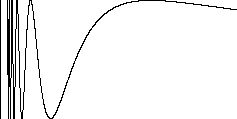
\includegraphics{varsavskilok.pdf}
% \caption[caption za v kazalo]{Dolg caption pod sliko}
  \caption[Primer vektorske slike.]{Relacije pokritja v trditvi~\ref{trd:pokritja} lahko prikažemo z grafom.}
  \label{fig:varsavski_lok}
\end{figure}

\begin{figure}[h]
  \centering
  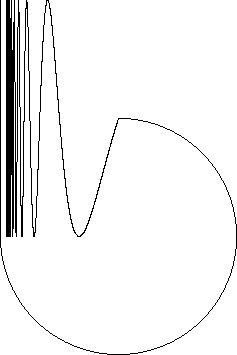
\includegraphics{varsavska_kroznica.pdf}
  \caption[Varšavska krožnica]{Slika prikazuje primer varšavske krožnice določene s predpisom $p$ iz definicije.}
  \label{fig:varšavski}
\end{figure}


\begin{definicija}\label{def:vk}
varšavska krožnica je topološki prostor, ki ga lahko definiramo na naslednji način:
$$S_W = \left\{\left(x, \sin\left(\frac{\pi}{x}\right)\right); 0 < x \leq 1\right\} \cup \{(0, y); -1 \leq x \leq 1\} \cup C,$$
kjer je C zvezna krivulja, ki povezuje točki $(0,1)$ in $(0,0)$ in ne seka preostalega dela Waršavske krožnice.
Množici, ki jo lahko parametriziramo na naslednji način:
\[ p(t) = \begin{cases}
  (t, \sin(\frac{\pi}{t}), & \mbox{ če $t \in (0, 1) $}\\
 (\cos(\frac{3\pi x}{2}-\frac{\pi}{2})+1, \sin(\frac{3\pi x}{2}-\frac{\pi}{2})-1). & \mbox{ če $t \in [1, 2]$}\\
  (0, 2t-5), & \mbox{ če $t \in (2, 3]$.}
  \end{cases}
  \]
\end{definicija}

\begin{trditev}
Varšavska krožnica je prostor Šarkovskega.
\end{trditev}

\begin{tikzcd}
A \arrow{d} \arrow{r}[near start]{\phi}[near end]{\psi}
& B \arrow[red]{d}{\xi} \\
C \arrow[red]{r}[blue]{\eta}
& D
\end{tikzcd}

\begin{proof}
Varšavsko krožnico $X$ lahko parametriziramo z zvezno bijektivno preslikavo $p:I \to X$. Naj bo $f: X \to X$ zvezna funkcija. Ker je funkcija $p$ bijektivna, je funkcija $\widehat{f} = p^{-1} \circ f \circ p : I \to I$ dobro definirana. Trdimo, da je funkcija $\widehat{f}$ zvezna. Ker je funkcija $p$ bijekcija, imata funkciji $f$ in $\widehat{f}$ enake periode. Ker je interval $I$ prostor Šarkovskega, je tudi $X$ prostor Šarkovskega. 

Prepričati se moramo samo še, da je funkcija $\widehat{f}$ res zvezna. Naj bo $t \in I$ poljubna točka intervala $I$ in naj bo $U \in I$ odprta krogla okoli točke $\widehat{f}(t) = (p^{-1} \circ f \circ p)(t)$. Množoco robnih točk krogle $U$ označimo z $A$. Velja $|A| \leq 2$. Ker ima $X$ lastnost $T_2$, so točke zaprte množice in zato je množica $X - p(A)$ odprta podmnožica prostora $X$, ki vsebuje točko $(f \circ p)(t)$. Povezano komponento množice $(f \circ p)^{-1}$, ki vsebuje točko $t$ označimo z $W$. Množica $W$ je odprta podmnožica intervala $I$, saj je funkcija $(f \circ p)$ zvezna. Sedaj obravnavamo množico $\left(p \circ \widehat{f}\right) (W) = (f \circ p)(W) \subseteq X - p(A)$. Ker je množica $W$ povezava s potmi, je vsebovana v tisti komponenti za povezanost s potmi množice $X-p(A)$, ki vsebuje $(f \circ p)(t)$. 
Prepričali se bomo, da je ta komponenta kar enaka $p(U)$. To je res, saj komponenta vsebuje $p(U)$ in ne more vsebovati nobene druge točke. Denimo, da vsebuje še kakšno drugo točko $x$. Potem vsebuje pot od $x$ do $p(t)$. Ta pot pa  
\end{proof}

\begin{figure}[h]
  \centering
  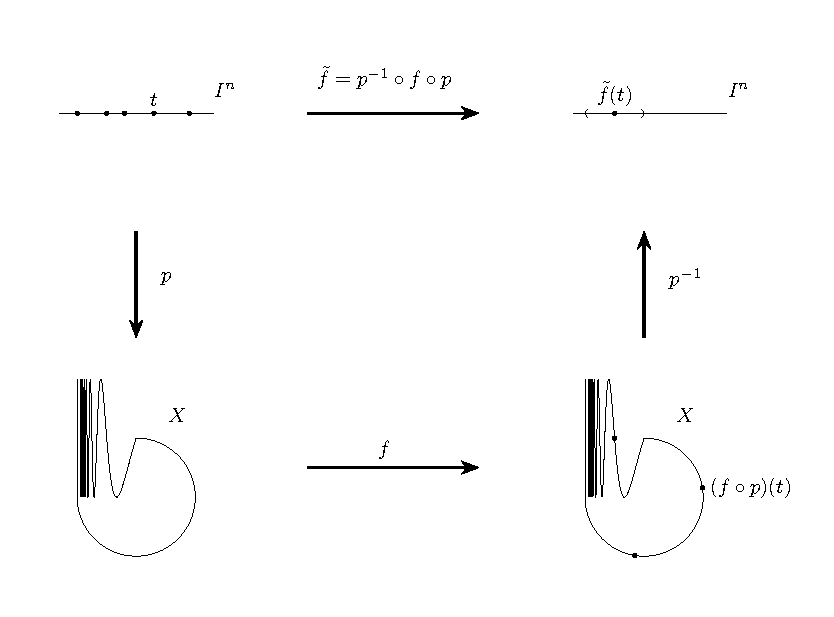
\includegraphics{vk-shark.pdf}
  \caption[Varšavska krožnica]{Slika prikazuje primer varšavske krožnice določene s predpisom p iz definicije.}
  \label{fig:varšavski}
\end{figure}

\end{document}